\chapter{System Architecture and Developed Mechanisms}

    As the main proposed goal of this work is the implementation of a system that complies with the ALTO working group's devised protocol, this chapter exhibits the planned software specifications needed to implement the system as a whole.

    Initial attention is given to the general architecture on the first section, with the goal of identifying key entities, their purpose, and how they interact among themselves.
    The following section will target the specification of ALTO resources, which can be considered the driving force behind the system, as they are what the client entities seek, and likewise what the ISPs wish to provide.
    The next section will focus on specifying the task of network status provision to an appropriate ALTO server, in such a way that a common interface exists among all entities that are able to increase the server's knowledge of the network's physical topology.
    Upon specified the way that network information is provided, the next section details how a given actor, such as an ISP administrator, can pre-process such information before it is forwarded to the server and available to clients.
    Finally, the task of multi-domain ALTO server synchronization and communication is specified in the form of required protocol extensions and needed mechanisms that allows the increase of a single ALTO server's knowledge space.

    \todo{add this : which includes the insertion of static ISP preferences or the abstraction of network entities as a means to dilute concrete topology details without forfeiting the usefulness the clients can retrieve from the processed resources}

\subsection{System Architecture}

    Figure \ref{fig:architecture-network} presents a high-level conceptual model of how the network information flows in a given ISP.
    Network data originates in the topology itself, and is gathered into a network information aggregator by the appropriate means - this aggregator defines an interface through which network data can be uploaded, and entities utilize it to provide the network data they have collected.
    These entities will use different means to gather different information, as the Internet consist of many different protocols and standards for network and resource information querying.
    For example, a node could deploy a daemon listening for Open Shortest Path First (OSPF) protocol packets to gather path cost information, and another using Simple Network Management Protocol (SNMP) to gather node property information.
    Obviously, since the interface simply defines how raw data must be formated to be accepted by the network information aggregator, the network administrator could use previously collected information that resides in a database and upload it as is.
    The network information aggregator serves as a hub for network administrators to process the raw network data that was collected by the previous tier, and transform it into ALTO resources ready to be accepted and distributed by the ALTO server.
    This task of network information processing is where ISP policies and preferences are injected via, for example, the abstraction of network entities with the aggregation of network addresses into PIDs, and the creation of cost maps which result from the transformation of network link information mixed with given ISP goals.
    If, say, the administrator wished to provide a cost map between network entities which aimed to reduce inter-network traffic, it would firstly aggregate endpoints into abstract entities with common properties, as an attempt not to share too much infrastructural information, and then use the provided network link information, attribute higher costs to undesired links, and transform it utilizing the Dijkstra's algorithm to create a shortest path map.
    Such map is then parsed as an ALTO resource and uploaded into the ALTO server with the access policies the administrator sees fit.

    As most software architectures, each new communication channel represents a possible attack vector and, attending to the critical security concerns posed in \ref{sssec:alto-security}, all pondered communication channels must be secure and reliable, as signified by the padlocks on the presented architecture.
    This implies that data communications within it must be resistant to being read or altered by outside parties, and the identity of the participating parties can be trusted and be made accountable.
    The identified communication channels must then have methods of maintaining data integrity in transit, user authentication and authorization, and communication confidentiality.

\begin{table}[!h]
\centering
\caption{Network node entities in the conceptual ALTO system representation}
\begin{tabular}{ | c | l |}
\hline
\textbf{Image} & \textbf{Description} \\ \hline
\raisebox{-.30\height}{
\includegraphics[width=8mm]{img/circle-white}} & Network node \\ \hline
\raisebox{-.30\height}{
\includegraphics[width=8mm]{img/circle-blue}} & Network node participating in a given overlay network \\
\hline
\end{tabular}
\end{table}

\begin{figure}[!h]
        \centering
        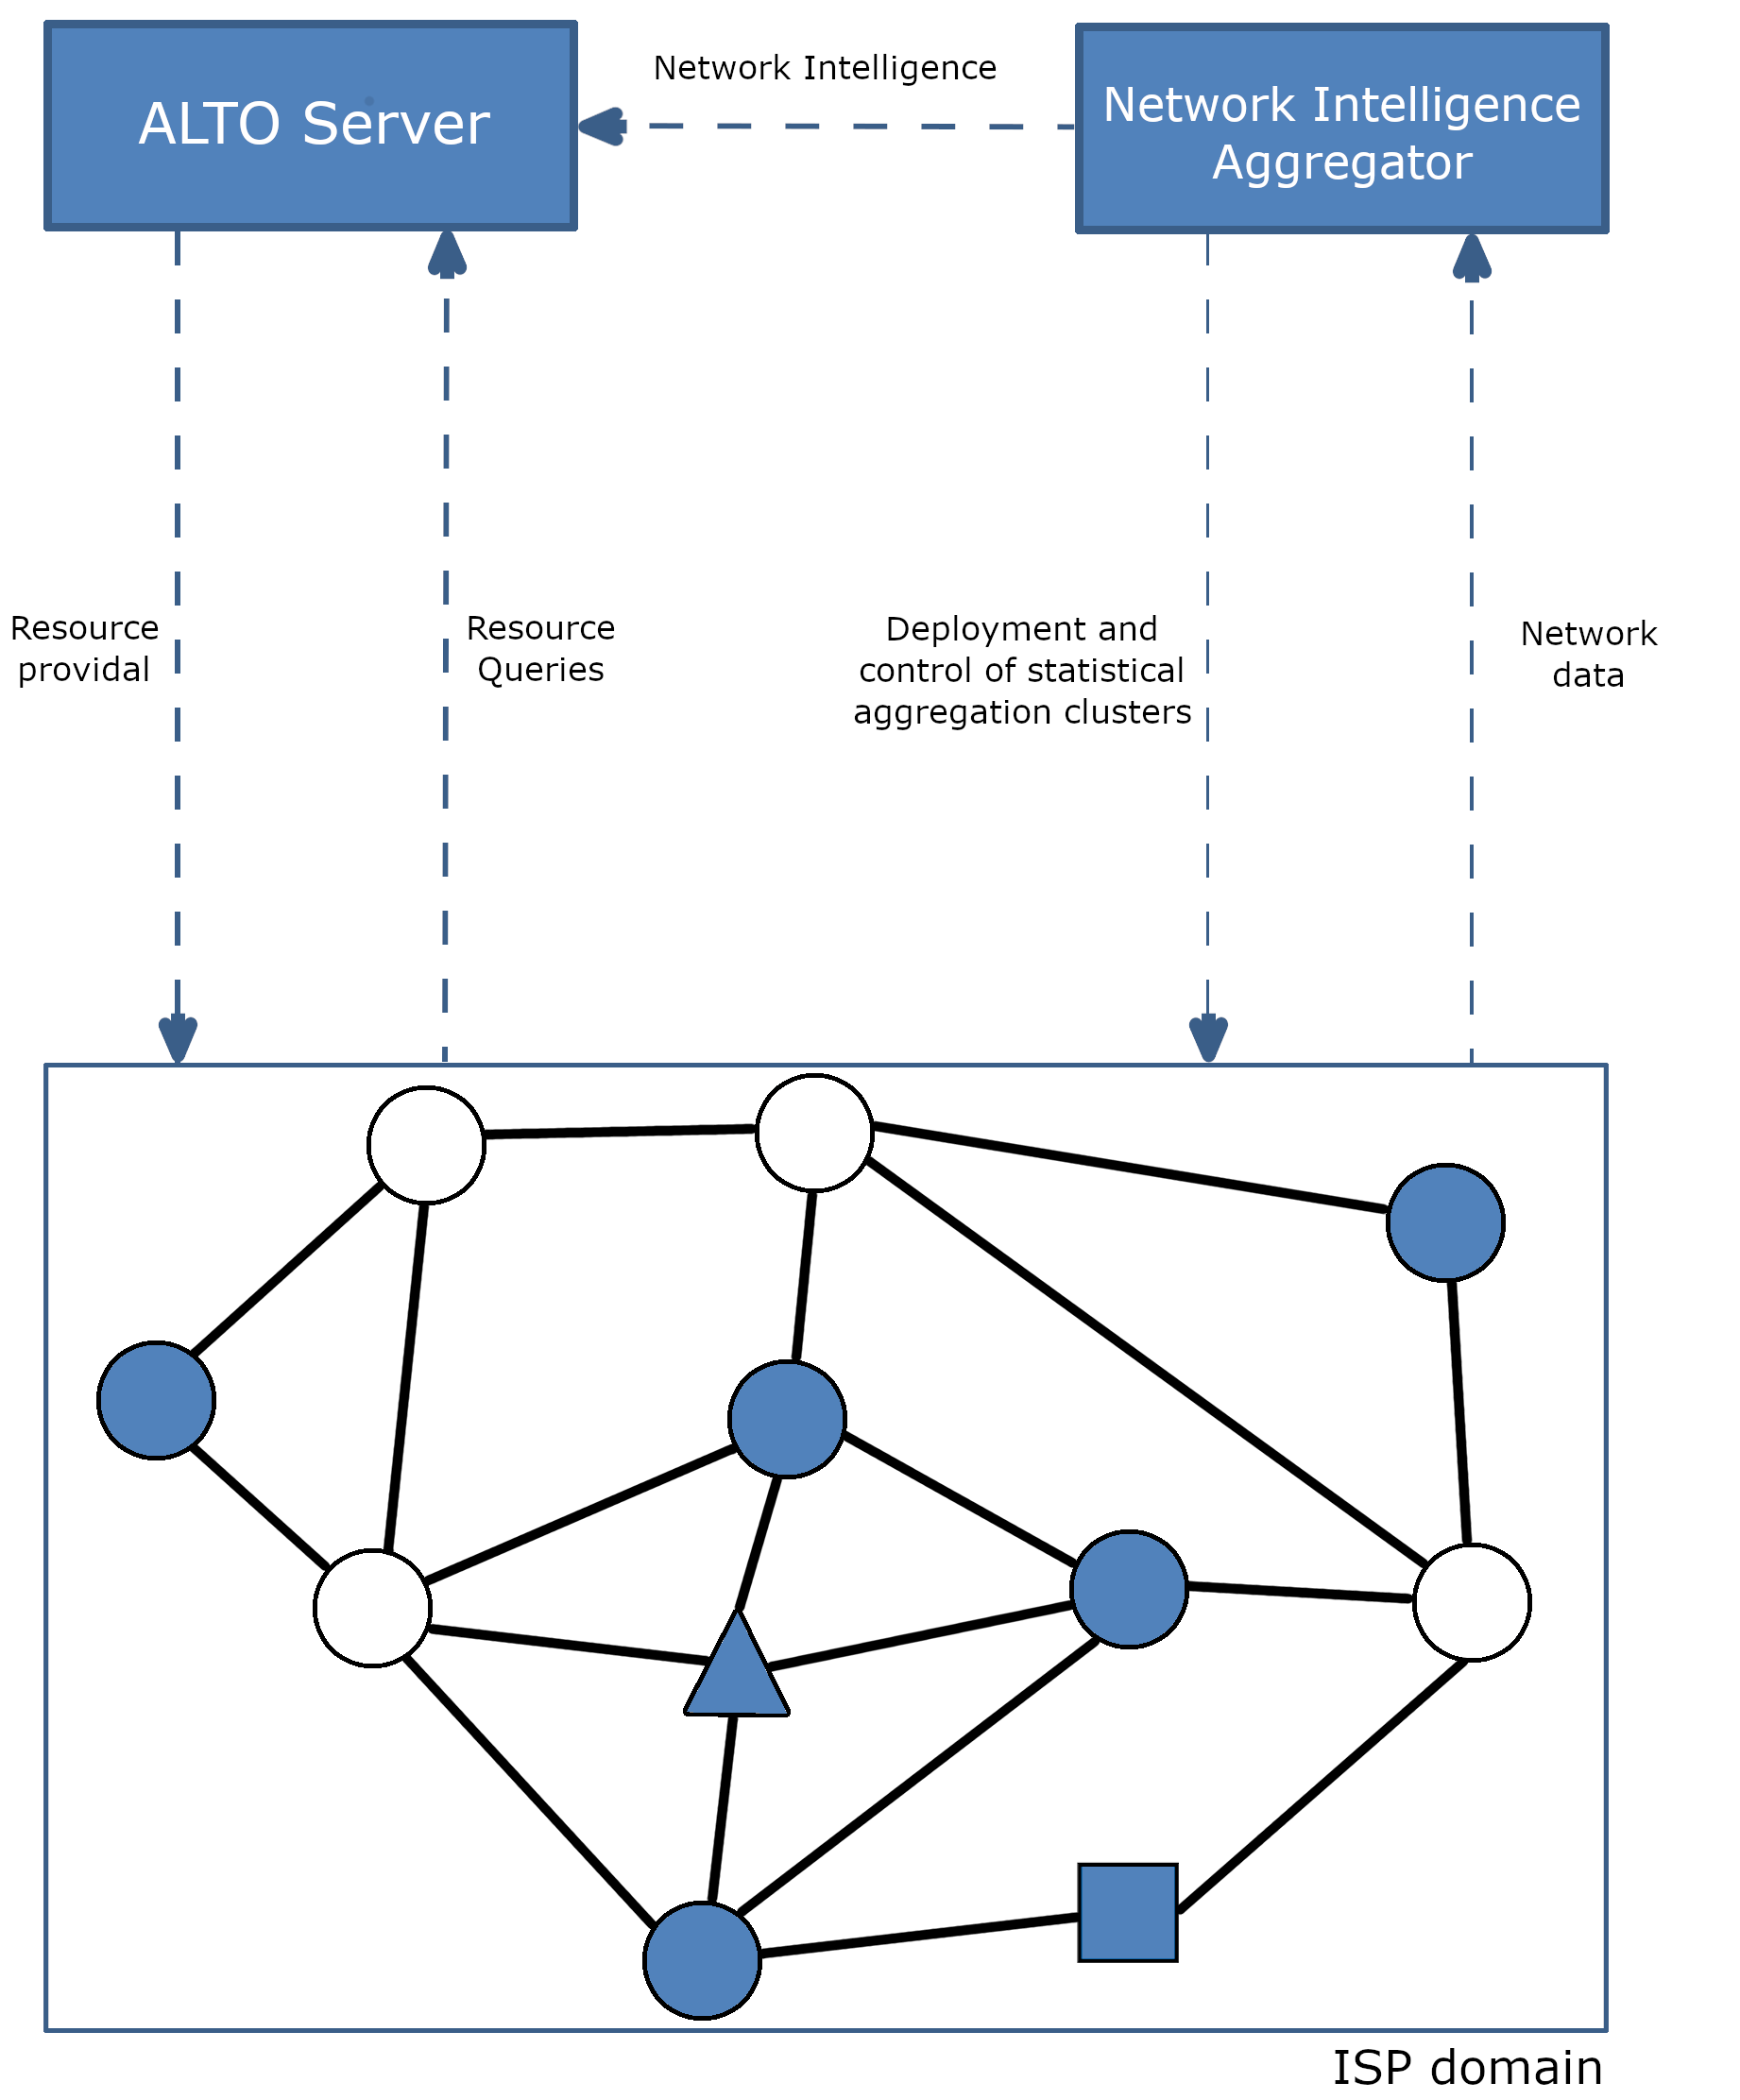
\includegraphics[scale=0.75]{img/architecture-network.png}
        \caption{Conceptual representation of the ALTO system of a given ISP}
        \label{fig:architecture-network}
\end{figure}

    More formally, Figure \ref{fig:macro-architecture} presents the proposed system architecture.
    One can identify the ALTO interface as a key component of the system, as it allows to bridge three different application layers - the ALTO resource consumer, the ALTO resource provider, and the network information aggregator, to be further specified in the following sections.

    The ALTO working group has extensively specified the ALTO protocol in regards to resource query, and the concrete implementation of this work will aim to comply to it.
    However, no resource provisioning protocol was, at time of writing, specified by the working group, nor was an interface been specified to allow network data to reach the ALTO server.
    It has been set as a work in progress, and the topic of network information supply sources was briefly discussed in \cite{alto-deployment-considerations}.
    The working group has grouped the tasks of raw network processing and supply into the role of the ALTO server.
    However, as can be seen in the proposed architecture, the roles were separated and an additional protocol proposed to bridge communication between them.
    This was made as an attempt to adhere to the philosophy of single responsibility, making the sole task of the ALTO server the management of ALTO resources.
    This aims to facilitate the independent development of the different roles, and make it easier to interchange implementations - this would make it particularly useful, for example, to deploy many ALTO servers in a cascade fashion whilst utilizing only a single network information aggregator.
    These are, however, only conceptually separated, and an implementation could, if it is more practical, merge the server and information provider roles into a single physical entity - which is similar to the architecture designed by the ALTO working group - if the conceptual roles and interfaces persist.

\begin{figure}[!h]
        \centering
        \includegraphics[scale=0.25]{architecture-macro.png}
        \caption{System architecture at a macro level}
        \label{fig:macro-architecture}
\end{figure}

\subsubsection{Role system}
\label{sssec:system-roles}

    As an access control measurement, the system will work with Role-based Access Control (RBAC) methods which, as the name states.
    Thus, every entity acting on the system must identify itself as a user, and a given user can have many roles.
    The ALTO resources - the main interest of this system as it is the data component requested by clients and managed by the servers - has associated to it an Access Control List (ACL), that maps, for a given set of roles and a special "catch all" role when none else apply, the list of user actions that are allowed to be performed to that resource.
    The available user actions are read, update and delete, meaning the ability to get, change the contents of, or remove the resource, respectively.
    This ACL is provided by the Network Information Aggregator whenever a new resource is inserted into the ALTO server.
    The ISP administrator that controls the aggregator not only then designs the resource itself - adding the information that it deems important whilst not too detailed to damage privacy - but also defining access control policies on that resource, which will be then applied by the server in future requests.

    Employing access control based on roles seems appropriate for this system since roles can be applied to, and thus group, many users, and indeed that seems to be applicable on real case deployments of the ALTO system - each given application can correspond to a group, and more intimate scenarios - such as a data center - can be grouped too.
    As a user can be conceded many roles, he can naturally act on the system with a role that fits the currently queried resource, if so applies.

    Access control mechanisms such as this will help mitigate security threats pertaining to the ALTO working group's architecture - e.g. having unwanted users reading or tampering with data - mechanism that is also based on roles can give better flexibility on access credence attribution, as well as better scalability since these credences can be applied of groups instead of managed on a user-by-user basis.
    However, for such mechanisms to be viable at all, authentication systems need to also be employed to help verify that the users are indeed who they are announcing to be, and nevertheless authentication seems to be a very important requisite of this system to mitigate spoofing security threats.

    Data breaches are not, however, totally mitigated with authenticity and access control mechanisms.
    After an entity gets a resource and acts outside the system, it becomes out of its control and these mechanisms cannot be employed.
    This means that there are no guarantees that the resources are shared outside of the system's domain and consequentially there are no security guarantees after that point.
    Because of this, privilege attribution by the ISP administrators not only give credence to do a certain action, but also imply that trust exists that these users will not be improper with the given resources and they won't thus share it with other users with improper credence.


\subsubsection{Resource Consumer}

    An ALTO resource consumer is materialized in the architecture in the form of an ALTO client, which can be any entity who is able to interface with an ALTO server to query for ALTO resources.
    Whilst the ALTO working group was initially devised to help increase traffic localization via the sharing of network information, it now has an increased scope where an ideal client is any application which generates network traffic and would be able to optimize it with aid from an oracle entity with privileged network information.
    Thus, an ALTO client is fit to be implemented in P2P applications, and could be embedded in a P2P client itself to help with picking neighbouring and content providing nodes, or on a tracker that would accomplish the same goal on behalf of the querying peer.
    Likewise, nodes which are unable to optimally select between other nodes, such as CDN edge nodes or content mirrors, could also benefit from oracle guidance, and thus qualify as appropriate ALTO clients.

    Figure \ref{fig:p2p-communication} exemplifies how a cooperative P2P application would, acting as an ALTO client, interact with the ALTO server to retrieve relevant network resources to aid their application choice of what candidate peer to consume a service from.
    Firstly, a network map is retrieved to help group endpoints into groupings, and afterwards a cost map is retrieved filtering only the querying peer as source, candidate peers as destinations, and the routing cost and bandwidth cost matrices.
    Acting on this information, the peer chooses the candidate that gives a good balance between ISP routing cost and path bandwidth, making a decision that should ideally benefit both them and the ISP that provided the information.

    Figure \ref{fig:p2p-tracker-communication} is similar to the previous example, meaning it relates to a P2P application, but this time the application-level traffic optimization is made in a way that is transparent to the P2P client.
    As a choice to purely localize traffic, as this alone can bring plenty of benefits to both layers, and as a means to minimize protocol modification, it is the tracker that serves as an ALTO client.
    Whenever a request is made by a P2P client to retrieve peers serving a given data chunk, the tracker first consults with the ALTO server and retrieves its network map that groups peers within administrative domains - inside the providing ISP's domain, thus the local network, and outside administrative domains.
    The tracker could use a very simple algorithm to filter out of its candidate pool candidate peers outside the local domain if results inside it exist.
    After packaging a reply to the P2P client, the protocol acts normally and traffic could be successfully localized.

    On the same vein, Figure \ref{fig:cdn-communication} exemplifies how this time a cdn controller would use the system to better help its decision in matching CDN clients to an edge server on their system.
    To do this, it retrieves a property map to query for server status information, and subsequently retrieves a cost map to query for path information between the CDN client and the candidate edge servers.
    Having all the relevant server status information, e.g. available processing and storage resources, and path properties, e.g. max bandwidth, latency, packet loss, the CDN controller is in a condition to more optimally redirect his client.

\subsubsection{Resource Provider}

    An ALTO resource provider is the ALTO server, an entity that possesses pre-processed network information in the form of ALTO resources.
    Its job is to store and manage such resources, and provide it to querying ALTO clients, and Integral to these responsibilities are also data validation and persistence.
    Conceptually, the ALTO server is seen as a single entity, but considering the sensible information that could be stored within it and the influence it has on shaping network traffic, it would not be uncommon for an ALTO server to have a knowledge domain correspondent to the ISP that owns it.
    Physically, though, the resource provider layer could consist of many interlinked ALTO providers with an increased coverage area of network knowledge.
    Means through which this could occur are further specified in section \ref{ssec:multi-alto}.

\subsubsection{Network Intelligence aggregation}

    The network intelligence aggregation layer is the layer that enables the translation of raw topological information - such as the physical attributes of network devices and connections - into processed, query-eligible network knowledge.
    To do so, a very important entity, perhaps the heart of the system as a whole, is the network state provider, which is the supply of network information that is injected, through a network state provisioning protocol, into a network information aggregator.
    This latter entity is then responsible for providing the ALTO resource provider layer with valid information after the raw topological data has been processed - this includes the calculation of optimal paths, the abstraction of network entities, or the injection of static ISP preferences.
    This pre-processing stage requires input from an ISP administrator, responsible for acting on the best behavior or the ISP from which the raw topological data originates - by interacting with the network information aggregator the administrator acts on this network information hub to retrieve from the database a history of retrieved network information, and afterwards manipulate this information to create ALTO resources to its liking - this is where data is transformed utilizing the algorithms the admin deems fitting, and transforms the raw data to be publishing ready, meaning that it contains an acceptable amount of abstraction not to compromise topological privacy.
    Finally, the admin defines important meta data that identifies the resource, and defines the access control list to be enforced by the ALTO server.

\subsubsection{Resources}
\label{ssec:alto-resources}

    ALTO resources are pieces of network information which are provided by an ALTO server and consumed by ALTO clients that ideally would use such information to aid their application-level traffic decisions.
    All ALTO resources can be separated into the following:

\begin{itemize}
        \item \textbf{Meta information}: data which regards to the resource's profile, that enable the client's ability to interpret and cross-reference the network data within.
            Following suit to the defined protocol, meta information contains the resource's name, if applicable, version, resource dependencies and cost details - enclosed cost modes, metrics, and descriptions.
            Finally, belonging to the meta section of the resource's information is the resource's ACL which, to a given set of roles, specifies what action those roles can perform on the resource.

        \item \textbf{Network status information}: data structures that give a characterization of the ALTO Server's vision of a network. Concretely, these can map network properties to a node (such as the connection types of their interfaces, or their geographical location), they can aggregate many network addresses to a single identifier, or they can map properties to a node link or end-to-end path (such as link or cumulative routing costs).
\end{itemize}{}

    Meta information can be seen as a resource's header, containing data that regards to the network status and helps better handle it.
    Following the defined protocol \cite{alto-protocol}, this field includes the resource's name for all resources which is needed for identification, and all other fields are dependant on the type of resource: at this version of the protocol, only network maps are version-able, allowing ISPs to reference different versions of a network map as this is updated; cost information is, naturally, only applicable to cost maps, and gives insight on how the numeric costs are to be interpreted, i.e. what their mode and metrics are, and what description it has.
    Finally, extending to the protocol is the addition of an ACL as a solution to access control needs.
    An ACL is defined as a matrix, with each entry defining a user role and actions - discussed in \ref{sssec:system-roles} - as a restriction on what a given user was given clearance to do.

    The network status information of a network map groups endpoint addresses into a single PID as a text literal.
    Akin to the ALTO protocol \cite{alto-protocol}, accepted endpoint address protocols include IPv4 and IPv6, utilizing a 32 bit long bitmask to identify a subnetwork.
    Similarly, support for aggregation of MAC addresses was added, with a 48 bit long bitmask to identify address ranges, similar to the IP variant.
    Additionally, generic overlay IDs can be added with the key priv:X - meaning private scheme - where X is the qualified name - this naming scheme was adapted from the endpoint property map's specification for additional property names, for semantic consistency.
    As endpoint addresses utilizing this scheme can be anything, the their interpretation is also left to the client - for example, if a server defines that PID aggregator of priv:my-overlay can use regular expression to specify address ranges, a pre-agreement must exist with a client.
    Of course, if a given addressing scheme besides the previously mentioned ones becomes popular, it could afterwards become part of the specification, but the existence of a private addressing scheme with liberal usage gives liberties outside of the protocol, if so are needed.
    A valid network map must unambiguously map every address in the domain range to a single PID, and whenever multiple matches occur wins the longest prefix match.
    As the custom addressing schemes let the network mad be interpreted in an undefined way by the protocol, the server cannot properly assert to the matching validity, and thus default protocol addressing schemes for network maps should be preferred, as semantic validity in private addressing schemes is not checked.
    Table \ref{table:networkmap-example} provides an example network status component of a network map within the topology in Figure \ref{fig:example-topology-boundary}.
    Three PIDs are given, each taking portion of an IPv4, IPv6, MAC, and custom overlay address range.
    The private address scheme groups users in regards to their private overlay ID, and it can be seen that nodes with ID 1, 3, and 4 are grouped to a single PID, which we can see belong inside the ISP domain.
    Lastly, nodes 2 and 5 are given different PIDs as they reside outside the ISP domain but are reachable through different peering points.
    The ISP could thus leverage the network map to define domains of locality, as well as defining two different external groups, as these two associated nodes are reachable through different peering parameters.

\begin{table}[]
\caption{Example network status information of a network map}
\begin{tabular}{llllc}
PID  & IPv4          & IPv6                  & MAC                  & \multicolumn{1}{l}{priv:my-overlay} \\
PID1 & 10.20.3.0/24  & \multicolumn{1}{c}{-} & D0-9F-BF-2A-00-00/32 & [1, 3, 4]                           \\
PID2 & 10.20.3.10/25 & \multicolumn{1}{c}{}  & D0-9F-BF-2A-FE-00/40 & 2                                   \\
PID3 & 0.0.0.0/0     & ::/0                  & 00-00-00-00-00-00/48 & 5
\end{tabular}
\label{table:networkmap-example}
\end{table}

    A cost map consists of a list of cost map matrices, with each matrix setting pairwise values between an origin entity and a destination entity.
    If it is a standard cost map, these entities are represented by PIDs that can be cross-referenced from a network map which this resource depends on, and if it is an endpoint cost map, these entities are endpoint addresses which, similar to network maps, include IPv4, IPv6, MAC and private endpoint types.
    A matrix must specify the type of cost represented with both their cost type and cost mode, with available options being the ones specified in \cite{alto-cost-metrics(draft)}.
    Optionally, a cost matrix can specify calendar information about that matrix - similar to the current work in \cite{alto-calendar-cost-map(draft)} -  which signifies that besides having single-value costs - which are obligatory for any cost matrix - it also contains a time-sensitive list of costs that must be interpreted according to the calendar information provided.
    Table \ref{table:costmap-example} provides an example of cost matrices within a single cost map within the topology in Figure \ref{fig:example-topology-boundary}.
    As can be seen, a generic "routingcost" cost matrix - whose value increases with the associated costs of transferring data through that path, and derived as the ISP best sees fit - lets the ISP communicate routing preference to the client - costs within the ISP domain, i.e., from and to PID1, incur minimal cost, whereas paths that originate locally and target PID2 or PID3 - both utilizing peering links - are less preferable, with the former being two times less preferable than the former.
    A "packetloss" cost matrix is also provided, with the ISP applying preceding probing measurements between endpoints and averaging the values within PID groupings.
    In this case, locality is correlated with more reliable communications, and in situations where outside service is required, the cost matrix provides insightful information to help select the better peering connections.
    Finally, a "bandwidth" cost matrix can be seen, with the ISP applying probing measurements, topological insight, as well as collected feedback of previous application connections that occurred between endpoints to deduce theoretical available bandwidth between target points.
    Additionally, the inclusion of cost calendar capabilities to the cost matrix enables users to get a chronological view of bandwidth availability as rush hour arrives, with the single value cost being updated to the present time if a decision needs to be made only considering the current time.
    Note that, if more applicable, the ISP could've chosen to - in alternative or addition to - provide an endpoint cost map, which instead of having costs between groupings specifies endpoints.
    In this particular case, an ISP could've preferred to use groupings as a means to increase topological abstraction and concluded that the groupings can achieve functionally similar results.


\todo{remove link 2-5}
\begin{figure}[!h]
        \centering
        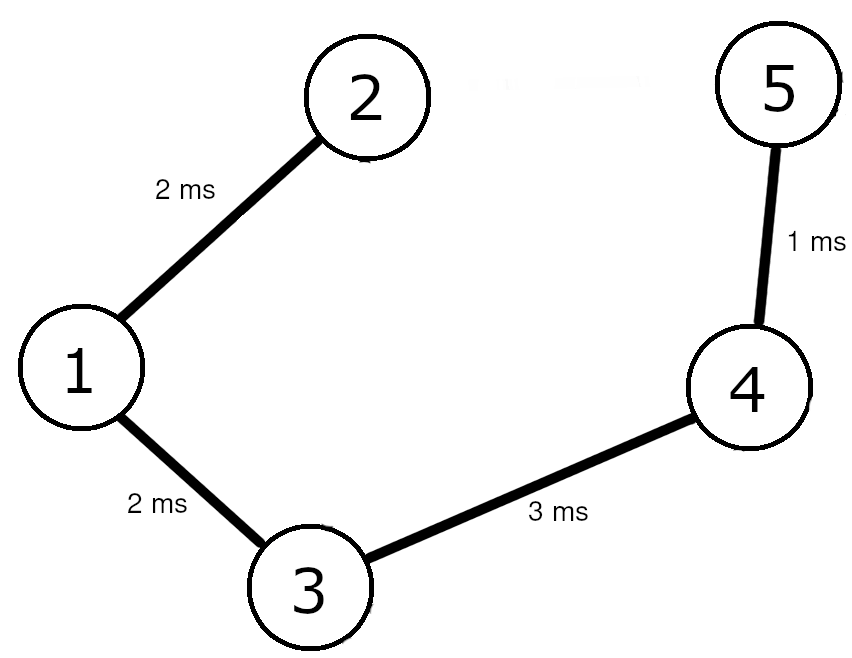
\includegraphics[scale=0.75]{img/topology.png}
        \caption{Example network topology with ISP boundary}
        \label{fig:example-topology-boundary}
\end{figure}

    The network status information of an endpoint property map stores the property information of a given endpoint.
    The ALTO working group's protocol specification \cite{alto-protocol} does not directly specify what kind of properties are pondered for this map.
    Following the same design pattern used for the other specified resources, the endpoint property map will have a set of defined properties with associated semantics, and all other properties can be added with the "priv" prefix to designate private properties outside of the considered domain, and thus all semantics and validation rules don't apply.
    Much like the other resources, an endpoint can be identified by an IPv4, IPv6, MAC or private overlay address, and the pondered properties are PID value, geographical coordinates, connection type (fiber, adsl, etc), server footprint information (total ram, storage, and processing power), and server status information (what part of the footprint information is currently available).
    In practice, a given property could be promoted from a private type to one pondered in the protocol and have a resulting official semantic and validation rules.

    Finally, as a means to facilitate resource divulgence from servers to clients, there is also included the specification of an Information Resource Directory (IRD), that is based from the ALTO working group's protocol specification.
    An IRD can also be thought of as a resource, but instead of sharing network information it serves as an index of the available resources that a given server provides.
    Each server must provide a single IRD, and it contains as many resource attributes as the amount of attributes it provides.
    Each resource attribute must contain the resource's ID and its HTTP media type and, if applicable, their capabilities, accepted input media types, and dependent resources.
    The capabilities identifies, if existing, the cost and property types that are used - being indexed by their unique name, this allows for these to be cross-referenced on further protocol exchanges without need to repeat information.
    Additionally, the resource's capabilities also serve to indicate what resource functionality extensions are enabled - currently applicable for cost maps only, it serves to signal if the cost map has calendared costs, if it accepts input filters, or if multiple cost matrices can be requested at once.
    Two additions are made to the working group's specification - firstly, a description field, which for each resource attribute gives a brief description of what it is about, as it could facilitate resource selection since such a description could go into detail about appropriate usage guidelines of that resource and suggested use cases; finally, the resource's ACL, letting a user know beforehand what credences he has in relation to the server's resources - being a crucial part of metadata of the resource, it seems fitting to go into the IRD, and has the added benefit of giving the user this crucial piece of information without him having to make resource requests just to, by server reaction, figuring out what he can and cannot do.

    Further formal specification is not made as it has been extensively done in the ALTO protocol \cite{alto-protocol}, and the proposed system is compliant to it whilst extending upon the design.

\subsection{Network status provision}

    Before ALTO resources are provided into the ALTO server by the Network Information Aggregator, the latter needs himself to be provided with raw network status information.
    The ALTO working group has discussed possible sources of raw topological information, including protocols like IGP, BGP, SNMP, or NETCONF, or databases like the Traffic Engineering Database (TED) or Label Switched Path Database (LSPD) \cite{alto-deployment-considerations}.
    A protocol needs to exist to interface between the entities that collect and provide the raw topological data, and the Network Information Aggregator that processes it and provides it to the ALTO server.


\todo{communication diagrams}
\todo{resources - source name, origin measurement time, description, endpoint/pair of endpoints, measurement}
\todo{interface}

\subsection{Network intelligence preprocessing}

\todo{communication diagram}

\subsection{Server discovery}

\subsection{Resource Filtering}

\subsection{Inter-server communication}

    \todo{add img/topolgy.png but more complex to showcase multi domain problem}

    A glaring gap in the working group's base ALTO protocol is its single administrative applicability domain.
    Meaning, an ALTO server is managed by a single administrative entity - likely an ISP - and its knowledge domain is limited by the network topology details that the entity wants to share.
    In the attempt to fix the server's inability to provide network status information outside its domain, this section overviews mechanisms that enable inter-server communication as a means to expand the capabilities of each domain.

    Firstly, consider how efforts for full resource synchronization could be taken.
    These would be similar to data synchronization mechanisms employed by popular databases to ensure consistency across several server replicas, and could increase availability as well as the serviceability of content nearby clients.
    However, it does not seem to fit this use case - for starters, if all data were to exist redundantly on all servers, that would defeat the purpose of having many administrative domains and thus a single server architecture would suffice; secondly, the architecture is inherently designed to work within a trust domain of selected clients, and because of it the servers may not even be comfortable with sharing all of its information within other domains to begin with, limiting replication strategies; thirdly, accounting for the amount of users acting on the ALTO system, better scalability could be achieved with a distributed solution that limits information within set boundaries.
    Accounting for these reasons, an inter-server synchronization protocol was designed for servers to negotiate information exchange among themselves.

\todo{communication diagrams}

\label{ssec:multi-alto}
